% !TEX program = xelatex
\documentclass[11pt, aspectratio=169]{beamer}

\usepackage{fontspec}
\usepackage[english]{babel}

% Set default/Latin font to Sans Serif in the main (rm) and sans (sf) slots for Beamer
\babelfont{rm}{Noto Sans}
\babelfont{sf}{Noto Sans}

\usepackage{amsmath}
\usepackage{booktabs}
\usepackage{graphicx}

% --- KNUST THEME CONFIGURATION ---
\usetheme{Madrid}
% Define KNUST Official Colors
\definecolor{knustgreen}{RGB}{0, 107, 63}
\definecolor{knustgold}{RGB}{253, 200, 47}

\usecolortheme[named=knustgreen]{structure}
\setbeamercolor{title}{bg=knustgreen, fg=white}
\setbeamercolor{frametitle}{bg=knustgreen, fg=white}
\setbeamercolor{block title}{bg=knustgreen, fg=white}
\setbeamercolor{block body}{bg=knustgreen!10, fg=black}
\setbeamercolor{item}{fg=knustgold!80!black}

% Remove navigation symbols for a cleaner look
\setbeamertemplate{navigation symbols}{}

\usepackage[backend=biber,style=authoryear]{biblatex}
\addbibresource{references.bib}


% Additional packages for Timeline
\usepackage{pgfgantt}

\title[Pediatric Counting Defense]{Making the Invisible Child Visible}
\subtitle{Automated Pediatric Census via Allometric Scaling \& Neuro-Symbolic Tracking}
\author[Peter \& Fafali]{Peter Amoah Mensah (3457122) \and Fafali Dorkunor (3455022)}
\institute[KNUST]{
    Department of Mathematics \\
    Kwame Nkrumah University of Science and Technology
}
\date{April 2026}

\begin{document}

% 1. Title Page
\begin{frame}
    \centering
    
\includegraphics[width=2cm]{images/KNUSTLogo.png} \\
    \vspace{0.2cm}
    \titlepage
\end{frame}

% 2. Background
\begin{frame}{Background: The Chaos of the OPD}
    \begin{columns}
        \begin{column}{0.55\textwidth}
            \textbf{The Clinical Reality in Ghana:}
            \begin{itemize}
                \item Hospitals like Komfo Anokye Teaching Hospital (KATH) experience overwhelming daily foot traffic.
                \item Accurate pediatric counts are critical for triaging, allocating nurses, and managing vaccine inventories.
                \item \textbf{Current State:} The Lightwave Health Information Management System (LHIMS) successfully logs registered adults, but struggles with the sheer volume of unregistered accompanying dependents.
                \item \textbf{The Consequence:} Resource misallocation and severe operational bottlenecks during peak hours.
            \end{itemize}
        \end{column}
        \begin{column}{0.45\textwidth}
            \centering
            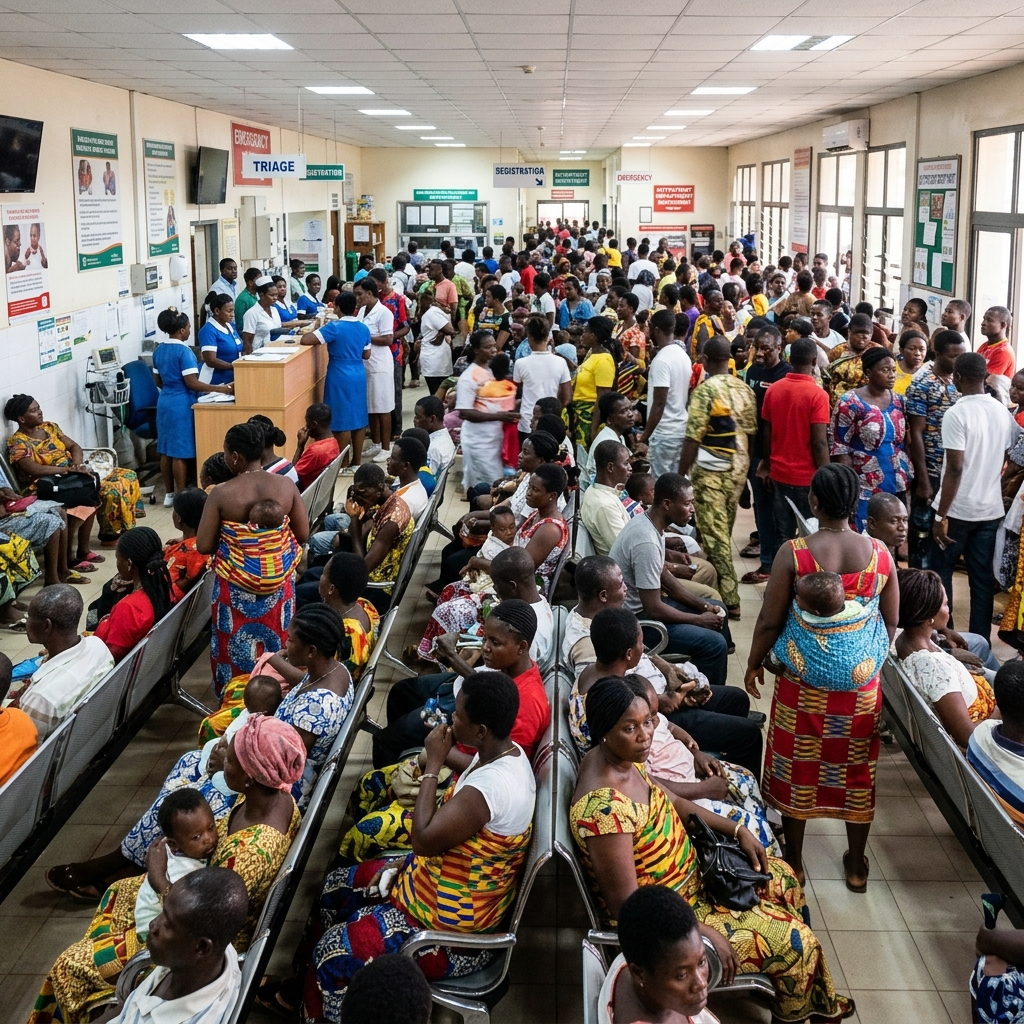
\includegraphics[width=\textwidth]{images/ghana_opd_crowd.png}
        \end{column}
    \end{columns}
\end{frame}

% 3. Problem Statement
\begin{frame}{Problem Statement: The Invisible Child}
    \begin{columns}
        \begin{column}{0.5\textwidth}
            \textbf{The Geometric Failure:}
            \begin{itemize}
                \item LHIMS captures registered patients, but accompanying infants are statistically invisible.
                \item Standard AI (e.g., standard YOLO) suffers from \textbf{Non-Maximum Suppression (NMS)} failure.
                \item When a mother carries a child in an \textit{ntoma}, their bounding boxes merge. The child is erased as "visual noise."
            \end{itemize}
        \end{column}
        \begin{column}{0.5\textwidth}
            \centering
            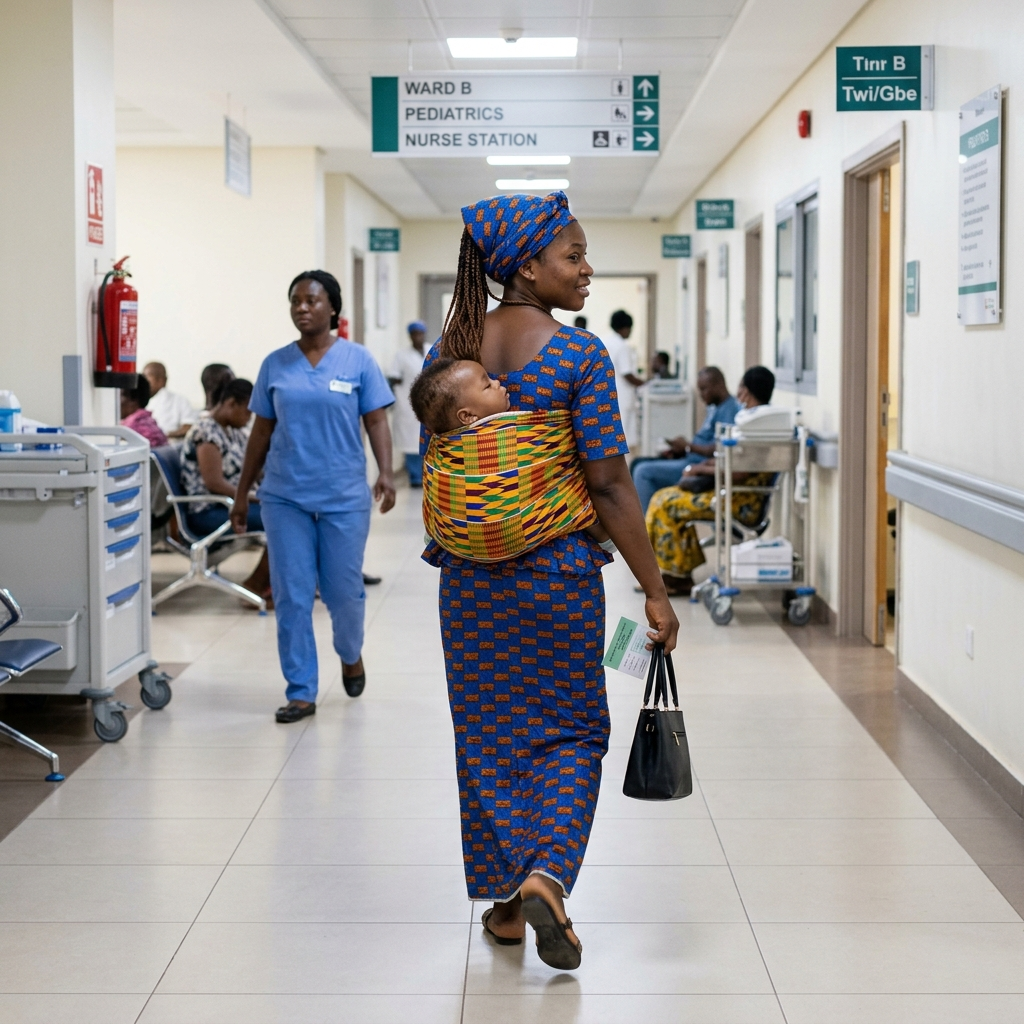
\includegraphics[width=\textwidth]{images/invisible_child.png}
        \end{column}
    \end{columns}
\end{frame}

% 4. Objectives
\begin{frame}{Objectives: Restoring Visibility}
    \textbf{Goal:} An automated, privacy-preserving framework to count pediatric visitors.
    
    \vspace{0.8cm}
    \textbf{Core Pillars:}
    \begin{itemize}
        \item \textbf{Mathematical Anthropometry:} Use biological scaling to bypass standard AI limits.
        \item \textbf{Spatial Inference:} Mathematically separate overlapping entities.
        \item \textbf{Neuro-Symbolic Tracking:} Deploy Kalman Filtering for unique patient IDs.
        \item \textbf{Edge Computing:} 100\% local processing for absolute medical privacy.
    \end{itemize}
\end{frame}

% 5. Methodology I
\begin{frame}{Methodology I: Allometry \& Spatial Invariants}
    \begin{columns}
        \begin{column}{0.5\textwidth}
            \textbf{1. Allometric Scaling ($R$):} \\
            We bypass facial recognition by using physical growth constants.
            \begin{equation*}
                R = \frac{H_{total}}{H_{head}}
            \end{equation*}
            \textit{Infants ($R \approx 4.0 - 6.0$) vs Adults ($R \approx 7.5 - 8.0$)} \\
            \vspace{0.3cm}
            \textbf{2. Spatial Occlusion Logic:} \\
            To override NMS limits, we apply conditional logic to detected bounding boxes ($h_1, h_2$):
            \begin{equation*}
                \text{IF } y_{h2} < y_{h1} \text{ AND } A_{h2} < A_{h1} \implies \text{Child}
            \end{equation*}
        \end{column}
        \begin{column}{0.5\textwidth}
            \centering
            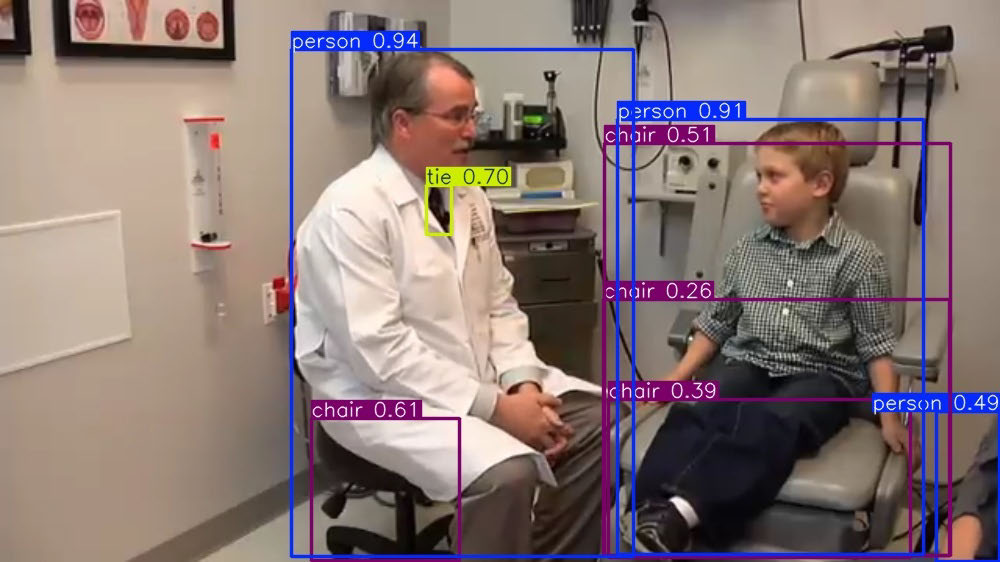
\includegraphics[width=0.9\textwidth]{images/fig-010.jpg} \\
            \vspace{0.2cm}
            \scriptsize{Comparative analysis: Standard NMS (left) vs. Specialized Spatial Fine-tuning (right).}
        \end{column}
    \end{columns}
\end{frame}

% 6. Methodology II
\begin{frame}{Methodology II: Tracking the Biological Entity}
    \begin{columns}
        \begin{column}{0.6\textwidth}
            \textbf{The Neuro-Symbolic Pipeline:}
            \begin{itemize}
                \item \textbf{Detection:} YOLOv11 extracts pixel-level precision masks.
                \item \textbf{Persistence:} How do we avoid double-counting if someone is occluded?
            \end{itemize}
            \textbf{Kalman Filter Prediction-Correction Loop:}
            \begin{block}{Prediction (Kinematics)}
                $\hat{x}_k^- = F\hat{x}_{k-1} + Bu_k$ \quad ; \quad $P_k^- = FP_{k-1}F^T + Q$
            \end{block}
            \begin{block}{Correction (Update)}
                $\hat{x}_k = \hat{x}_k^- + K_k(z_k - H\hat{x}_k^-)$
            \end{block}
            This mathematical engine ensures IDs remain persistent across complex spatial overlaps.
        \end{column}
        \begin{column}{0.4\textwidth}
            \centering
            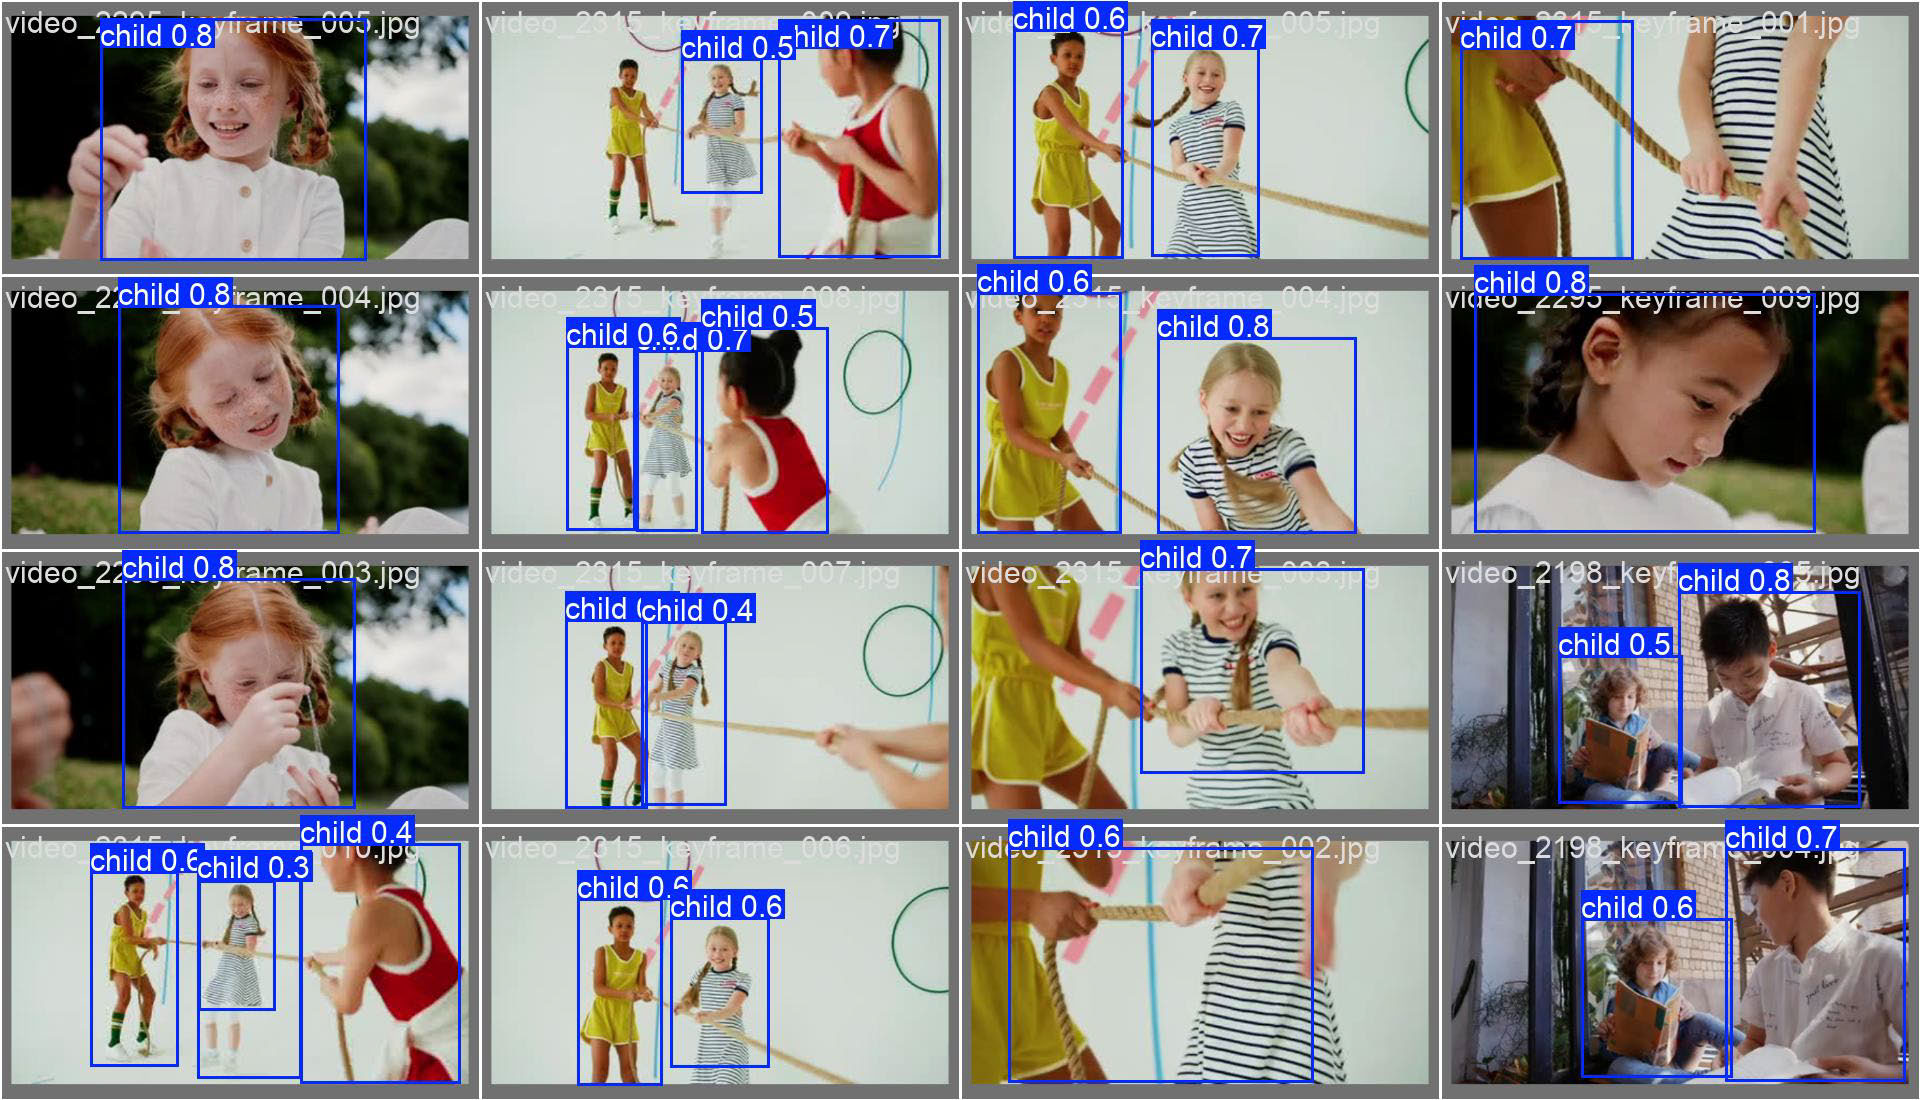
\includegraphics[width=0.9\textwidth]{images/fig-008.jpg} \\
            \vspace{0.2cm}
            \scriptsize{Training baseline: Diverse postures from the Child Detection Dataset.}
        \end{column}
    \end{columns}
\end{frame}

% 7. Justification
\begin{frame}{Justification: Why This Matters}
    \begin{columns}
        \begin{column}{0.5\textwidth}
            \textbf{Operational Efficiency}
            \begin{itemize}
                \item Eliminates manual clicker fatigue.
                \item Enables dynamic staff shifting during peak hours.
            \end{itemize}
        \end{column}
        \begin{column}{0.5\textwidth}
            \textbf{Ethical Medical AI}
            \begin{itemize}
                \item \textbf{Privacy:} 100\% Edge processing. No video saved.
                \item \textbf{Context:} Biological math solving a cultural geometric challenge.
            \end{itemize}
        \end{column}
    \end{columns}
\end{frame}

% 8. Expected Results
\begin{frame}{Expected Results: The Force Multiplier}
    \begin{columns}
        \begin{column}{0.5\textwidth}
            \textbf{Transforming Data into Action:}
            \begin{itemize}
                \item \textbf{High Accuracy:} Utilizing the Child Detection Dataset (CDD) for fine-tuning minimizes the Mean Absolute Percentage Error (MAPE) to $<10\%$.
                \item \textbf{Actionable Intel:} The framework outputs a clean numerical matrix of pediatric density.
                \item \textbf{Integration Ready:} This matrix acts as a plug-and-play data feed for the LHIMS dashboard.
            \end{itemize}
        \end{column}
        \begin{column}{0.5\textwidth}
            \centering
            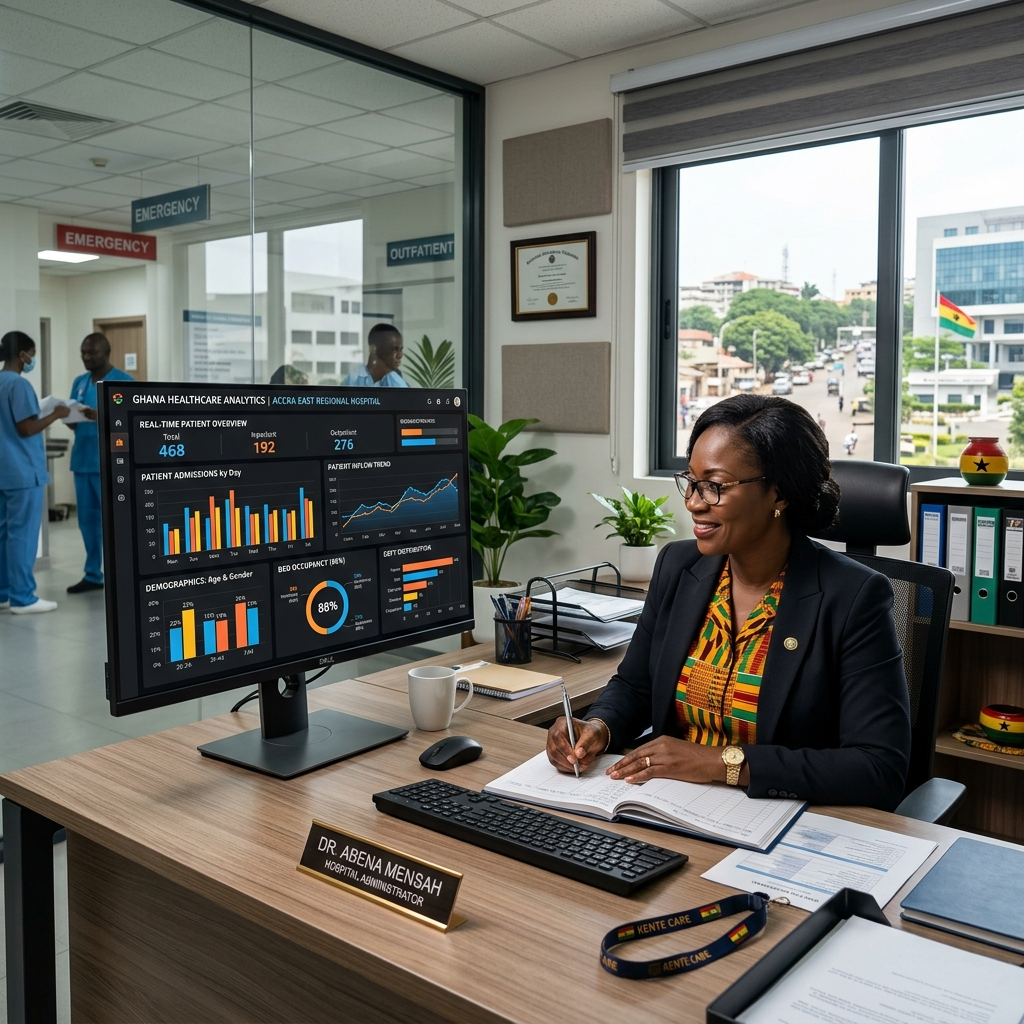
\includegraphics[width=\textwidth]{images/dashboard.png}
        \end{column}
    \end{columns}
\end{frame}

% 9. Timeline
\begin{frame}{Project Timeline}
    \begin{figure}[H]
        \centering
        \resizebox{\textwidth}{!}{
        \begin{ganttchart}[
            vgrid,
            hgrid,
            x unit=2cm,
            y unit title=0.6cm,
            y unit chart=0.6cm,
            title label font=\bfseries\footnotesize,
            bar label font=\footnotesize,
            group label font=\bfseries\footnotesize,
            bar/.style={fill=knustgreen},
            bar incomplete/.append style={fill=knustgold},
            group/.append style={fill=black},
            progress label text={},
            time slot format=isodate
        ]{1}{6}
            % Timeline Header
            \gantttitle{Project Timeline (Months)}{6} \\
            \gantttitlelist{1,...,6}{1} \\
    
            % --- Phase 1 ---
            \ganttgroup{Phase 1: Background \& Review}{1}{2} \\
            \ganttbar{OPD Data Scarcity Research}{1}{1} \\
            \ganttbar{Geometric Failure Analysis}{1}{2} \\
    
            % --- Phase 2 ---
            \ganttgroup{Phase 2: Methodology (Current)}{3}{3} \\
            \ganttbar{YOLOv11 Fine-Tuning}{3}{3} \\
            \ganttbar{Allometric Model Integration}{3}{3} \\
    
            % --- Phase 3 ---
            \ganttgroup{Phase 3: System Integration}{4}{4} \\
            \ganttbar{Edge Computing Deployment}{4}{4} \\
            \ganttbar{Kalman Filter Tracking}{4}{4} \\
    
            % --- Phase 4 ---
            \ganttgroup{Phase 4: Validation \& Testing}{5}{5} \\
            \ganttbar{CDD Dataset Testing}{5}{5} \\
            \ganttbar{MAPE Calibration}{5}{5} \\
    
            % --- Phase 5 ---
            \ganttgroup{Phase 5: Finalization}{6}{6} \\
            \ganttbar{Thesis Compilation}{6}{6}
            
            % Vertical line to show current progress
            \ganttvrule[vrule/.style={red, thick, dashed}]{Current Stage}{3}
        \end{ganttchart}
        }
    \end{figure}
\end{frame}


% 10. References
\begin{frame}{Selected References}
    \printbibliography
\end{frame}

\end{document}
